\documentclass[border=8pt]{standalone}
% Shared look for every circuit drawing: a sans-serif font (text and math),
% black lines, and white space around the picture.
\usepackage[T1]{fontenc}
\usepackage[scaled=0.95]{helvet}
\renewcommand{\familydefault}{\sfdefault}
\usepackage{sansmath}
\sansmath
\usepackage{amsmath}
\usepackage{array}
\providecommand{\ket}[1]{\lvert #1\rangle}
\newcommand{\truthtable}[1]{%
  \renewcommand{\arraystretch}{1.25}%
  \begin{tabular}{r|c|c}
    #1
  \end{tabular}}
\newcommand{\columnsum}[1]{%
  \renewcommand{\arraystretch}{1.1}%
  \begin{tabular}{@{}r@{}}
    #1
  \end{tabular}}

\usepackage{tikz}
\begin{document}
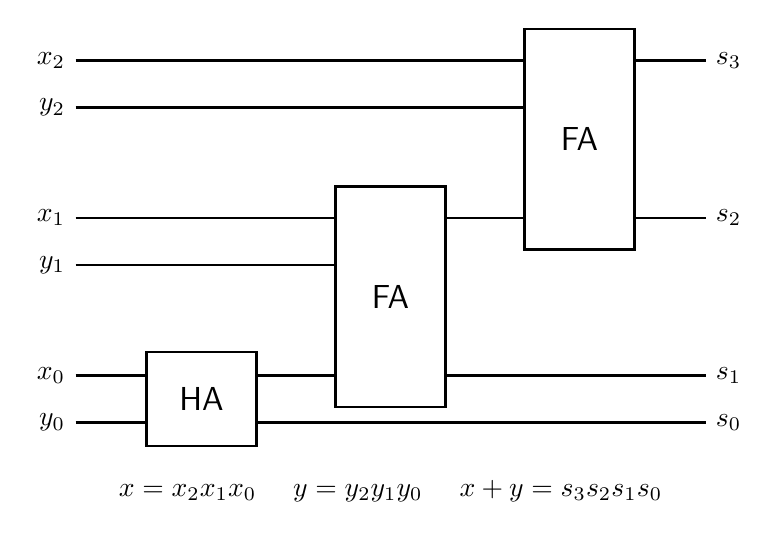
\begin{tikzpicture}[line width=0.9pt,
    block/.style={draw, minimum width=1.4cm, font=\large}]
  % input wires, from the 1s place (bottom) to the 4s place (top)
  \foreach \name/\y in {x_0/1.0, y_0/0.4, x_1/3.0, y_1/2.4, x_2/5.0, y_2/4.4}
    \node[left] at (0,\y) {$\name$};
  % the 1s place: a half adder (no carry comes in)
  \node[block, minimum height=1.2cm] (ha) at (1.6,0.7) {HA};
  \draw (0,1.0) -- (ha.west |- 0,1.0);
  \draw (0,0.4) -- (ha.west |- 0,0.4);
  % the 2s place: a full adder, with the carry from the 1s place
  \node[block, minimum height=2.8cm] (fa1) at (4.0,2.0) {FA};
  \draw (0,3.0) -- (fa1.west |- 0,3.0);
  \draw (0,2.4) -- (fa1.west |- 0,2.4);
  \draw (ha.east |- 0,1.0) -- (fa1.west |- 0,1.0);
  % the 4s place: a full adder, with the carry from the 2s place
  \node[block, minimum height=2.8cm] (fa2) at (6.4,4.0) {FA};
  \draw (0,5.0) -- (fa2.west |- 0,5.0);
  \draw (0,4.4) -- (fa2.west |- 0,4.4);
  \draw (fa1.east |- 0,3.0) -- (fa2.west |- 0,3.0);
  % the answer, one bit per place
  \draw (ha.east |- 0,0.4) -- (8.0,0.4) node[right] {$s_0$};
  \draw (fa1.east |- 0,1.0) -- (8.0,1.0) node[right] {$s_1$};
  \draw (fa2.east |- 0,3.0) -- (8.0,3.0) node[right] {$s_2$};
  \draw (fa2.east |- 0,5.0) -- (8.0,5.0) node[right] {$s_3$};
  \node[anchor=north] at (4.0,-0.2)
    {$x = x_2x_1x_0$ \quad $y = y_2y_1y_0$ \quad $x + y = s_3s_2s_1s_0$};
\end{tikzpicture}
\end{document}
